\documentclass[a4paper, 10pt]{report}
\usepackage[italian]{babel}
\usepackage[T1]{fontenc}
\usepackage[utf8]{inputenc}
\usepackage{charter}
\usepackage{amsmath}
\usepackage{amsthm}
\usepackage{amsfonts}
\usepackage{graphicx}
\usepackage{wrapfig}
\usepackage{tcolorbox}
\usepackage{fancyhdr}

\usepackage{geometry}
\geometry{a4paper, left=2cm,right=2cm,top=2cm,bottom=2cm}

\pagestyle{fancy}
\lhead{}
\chead{}
\lhead{\bfseries Fondamenti dell'informatica}
\rhead{\bfseries 16 ottobre 2019}

\begin{document}

\section*{\underline{Automi a stati finiti non deterministici}}
Un automa a stati finito non deterministico è una quintupla $<Q, \Sigma, \delta, q_0, F>$ dove:
\begin{itemize}
\item[-] $Q, \Sigma, q_0, F$ assumono lo stesso significato che hanno negli automi deterministici;
\item[-] $\delta$ resta la funzione di transizione, ma si definisce come: $\delta: Q$ x $\Sigma \rightarrow P(Q)$.
\end{itemize}

\noindent Poichè $P(Q)$ rappresenta l'insieme degli stati raggiungibili daopo aver letto un segno (più di uno essendo non deterministico l'automa), è possibile che $\delta(q, a) = \emptyset$. Il numero di stati raggiungibili è comunque limitato ($|\delta(q, a)| < \omega$ -> il numero di "fork" per stati successivi deve essere limitato).

Attualmente questi automi sono solo ideali, non ne esistono di reali. Praticamente sono macchine che operano in parallelo senza vincoli (per ogni "operazione" creo un nuovo stato dove la eseguo, così le eseguo tutte parallelamente).\\

\noindent Esempio:

\begin{center}
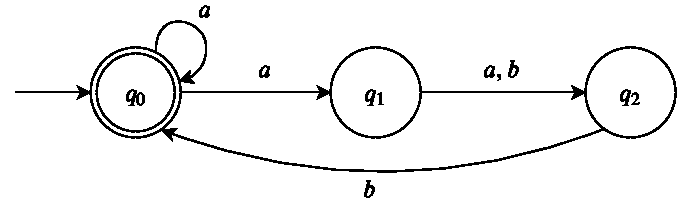
\includegraphics[scale=1]{16ottobre01.pdf}
\end{center}

\noindent La funzione $\hat{\delta}$ si ridefinisce come segue:

\begin{center}
$\hat{\delta}: Q$ x $\Sigma^* \rightarrow P(Q) = 
\begin{cases} 
\hat{\delta}(q, \varepsilon) = \{q\} & \\

\hat{\delta}(q, wa) = \bigcup_{p \in \hat{\delta}(q, w)} \delta(p, a)
\end{cases} $
\end{center}

\noindent Con $\{q\}$ si intende l'insieme singoletto che contiene solo $q$, mentre $\bigcup$ indica "unione di tutti".

\subsection*{Linguaggio accettato da un automa non deterministico}
Il linguaggio accettato da questo tipo di automi è definito come segue:
\begin{center}
$\mathfrak{L}(M) = \{ \sigma \in \Sigma^* $ | $ \hat{\delta}(q_0, \sigma) \cap F \ne \emptyset \}$  
\end{center}

\noindent Esempio:
Alfabeto $\Sigma = \{ a, b\}$; stringa da leggere: $aabb$.

\begin{center}
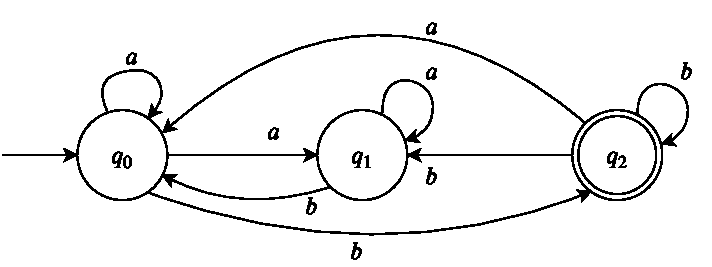
\includegraphics[scale=1]{16ottobre02.pdf}

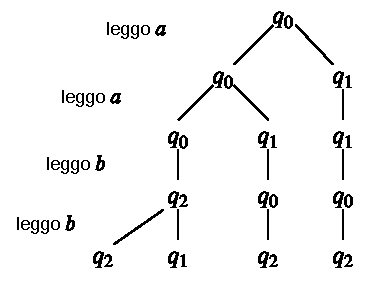
\includegraphics[scale=1]{16ottobre03.pdf}
\end{center}

\paragraph*{Teorema di Rabin - Scott (n. 1 1959)}
Sia $M = <Q, \Sigma, \delta, q_0, F>$ un automa a stati finiti non deterministico, allora esiste un automa a stati finiti deterministico $M'$ tale che $\mathfrak{L}(M) = \mathfrak{L}(M')$.

\begin{tcolorbox}[title=\textbf{Dimostrazione}]
Definiamo $M = <Q', \Sigma', \delta', q_0', F'>$ come segue:
\begin{itemize}
\item[-] $\Sigma' = \Sigma$;
\item[-] $Q' = P(Q)$;
\item[-] $q_0' = \{q_0 \}$;
\item[-] $F' = \{ P \subset Q : P \cap F \ne \emptyset\}$;
\item[-] $\delta'(P, a) = \bigcup_{p \in P \delta(p, a)}$, per $P \in P(Q)$;
\end{itemize}

Dimostriamo quindi, per induzione, che $\hat{\delta}(q_0, x)$ = $\hat{\delta}'(q_0', x)$:\\

Dimostriamo per induzione che $\forall \sigma \in \Sigma^{*}.\hat{\delta}(q_0, \sigma) = \hat{\delta}'(q_0', \sigma)$. \\ Caso base $|\sigma| = 0$:
	\[
		\hat{\delta}(q_0, \varepsilon) = \{q_0\} = q_0' = \hat{\delta}(q_0', \varepsilon)
	\]
	Passo induttivo: 
	\[
		\hat\delta'(q_0', \sigma a) = 
		\delta'(\hat\delta'(q_0', \sigma), a) = 
		\delta'(\hat\delta(q_0, \sigma), a) = 
		\bigcup_{P \in \hat\delta(q_0, \sigma)} \delta(P, a) = \hat{\delta}(q_0, \sigma a)
	\]
	Da questo consegue che:
	\[
		x \in \mathfrak{L}(M) \iff \hat\delta(q_0, \sigma) \cap F \neq \emptyset \iff \hat\delta'(q_0', \sigma) \cap F \neq \emptyset 
				\iff \hat\delta'(q_0', \sigma) \in F' \iff x \in L(M') 
	\]
	
\end{tcolorbox}

\noindent Esempio:\\

A partire dal seguente automa a stati finiti non definito, disegnare il relativo automa di Rabin - Scott.

\begin{center}
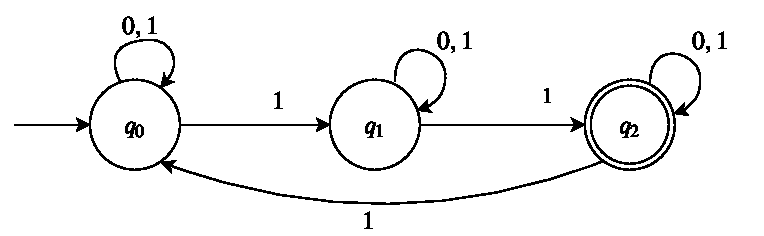
\includegraphics[scale=1]{16ottobre04.pdf}

(Automa non definito)

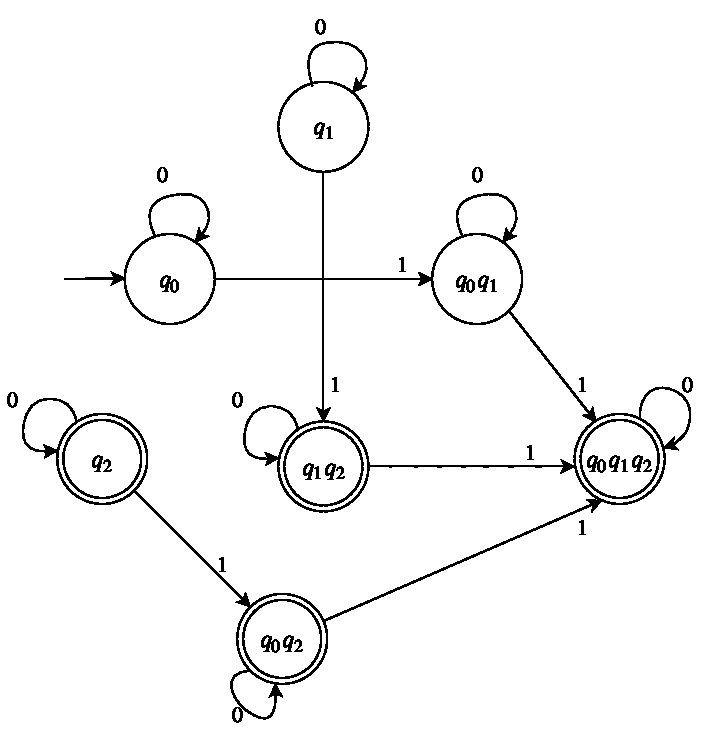
\includegraphics[scale=1]{16ottobre05.pdf}

(Relativo automa di Rabin - Scott)

\end{center}

\noindent Osservazioni:
\begin{itemize}
\item[-] L'automa di Rabin - Scott avrà $2^n$ stati (con $n$ = numero stati dell'automa non definito);
\item[-] Nello schema, l'ottavo stato rappresenta l'insieme vuoto (quindi non è rappresentato);
\item[-] $q_0 q_1$, ad esempio, rappresenta un insieme di stati;
\item[-] Un automa deterministico può essere visto come il caso speciale di quello non deterministico.
\end{itemize}

\section*{\underline{Automi a stati finiti non deterministici con $\varepsilon$ - transizioni}}
Un automa a stati finiti non deterministico con $\varepsilon$ - transizioni è una quintupla $<Q, \Sigma, \delta, q_0, F>$ dove:
\begin{itemize}
\item[-] $Q, \Sigma, q_0, F \subseteq Q$ assumono lo stesso significato che hanno negli automi non deterministici;
\item[-] $\delta$ resta la funzione di transizione, ma si definisce come: $\delta: Q$ x $(\Sigma \cup \{ \varepsilon\}) \rightarrow P(Q)$.
\end{itemize}

\noindent L’idea è che da uno stato è permesso passare ad un altro stato anche senza “leggere”
caratteri di input.\\

\noindent Si definisce $\varepsilon - chiusura$ la seguente funzione:
\begin{center}
$\varepsilon - chiusura = \{ q \in Q$ | $p \rightarrow Q\}$
\end{center}

\noindent In pratica, applicata ad uno stato, restituisce l'insieme degli stati raggiungibili da esso (compreso se stesso) tramite $\varepsilon$ - transizioni.\\

\noindent la funzione $\hat{\delta}$ si può definire come segue:

\begin{center}
$\hat{\delta} = 
\begin{cases} 
\hat{\delta}(q, \varepsilon) = \varepsilon - chiusura(q) & \\

\hat{\delta}(q, wa) = \bigcup_{p \in \hat{\delta}(q, w)} \varepsilon - chiusura[\delta(p, a)]
\end{cases} $
\end{center}

\begin{center}
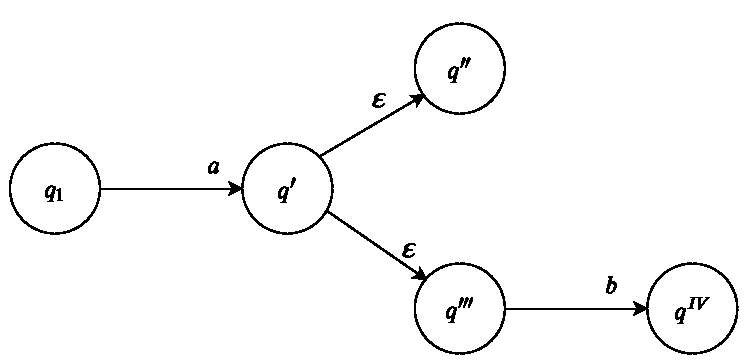
\includegraphics[scale=1]{16ottobre06.pdf}
\end{center}

\paragraph*{Teorema di Rabin - Scott (n. 2 1952)}
Sia $M = <Q, \Sigma, \delta, q_0, F>$ un automa a stati finiti non deterministico con $\varepsilon$ - transizioni, allora esiste un automa a stati finiti non deterministico $M'$ tale che $\mathfrak{L}(M) = \mathfrak{L}(M')$.

\begin{tcolorbox}[title=\textbf{Dimostrazione}]
Definiamo $M = <Q', \Sigma', \delta', q_0', F'>$ come segue:
\begin{itemize}
\item[-] $\Sigma' = \Sigma$;
\item[-] $Q' = Q$;
\item[-] $q_0' = q_0$;
\item[-] $F' = \begin{cases} 
F \cup \{ q_0\} & $se $\varepsilon - chiusura(q_0) \cap F \ne \emptyset \\

F & $altrimenti$
\end{cases} $;
\item[-] $\delta'(q, a) = \hat{\delta(q, a)}$;
\end{itemize}

Dimostriamo quindi, per induzione, che $\hat{\delta}(q_0, x)\cap F \ne \emptyset $ se e solo se $\hat{\delta}'(q_0', x)\cap F' \ne \emptyset$ (ipotesi induttiva $\forall x \in \Sigma^*\hat{\delta}(q_0, x) = \hat{\delta}'(q_0, x)$):\\

Caso base $|x| = 0$:
\begin{center}
$\hat{\delta}(q_0, \varepsilon) = \varepsilon$ - $chiusura(q_o) = \varepsilon$ - $chiusura(\delta(q_o, \varepsilon))$
\end{center}

Passo induttivo:
\begin{center}
$\hat{\delta}'(q_0', xa) = 
\bigcup_{p \in \hat{\delta}'(q_0', x)} \delta'(p, a) = 
\bigcup_{p \in \hat{\delta}'(q_0', x)} \hat{\delta}(p, a) = \bigcup_{p \in \hat{\delta}(q_0, x)} \hat{\delta}(p, a) = \bigcup_{p \in \hat{\delta}(q_0, x)} \hat{\delta}'(p, a) =
\bigcup_{p \in \hat{\delta}(q_0, x)} \varepsilon$-$chiusura(\delta(p, a)) = \hat{\delta}(q_0, xa)$
\end{center}

\end{tcolorbox}

\section*{\underline{Linguaggi regolari}}
Un linguaggio è regolare, quindi, se e solo se è accettato da un automa a stati finiti deterministico, da un automa a stati finiti non deterministico oppure da un automa a stati finiti non deterministico con $\varepsilon$ - transizioni.

Gli elementi base di un linguaggio regolare sono: $\emptyset$, $\varepsilon$, $a \in \Sigma$.

Se $R$ e $S$ sono espressioni regolari, allora anche $R + S$, $R \cdot S$ e $R*$ (== $R$, $RR$, $RRR$, ...).

\begin{tcolorbox}[title=\textbf{Dimostrazione (per induzione) grafica}]

Caso base:

\begin{center}
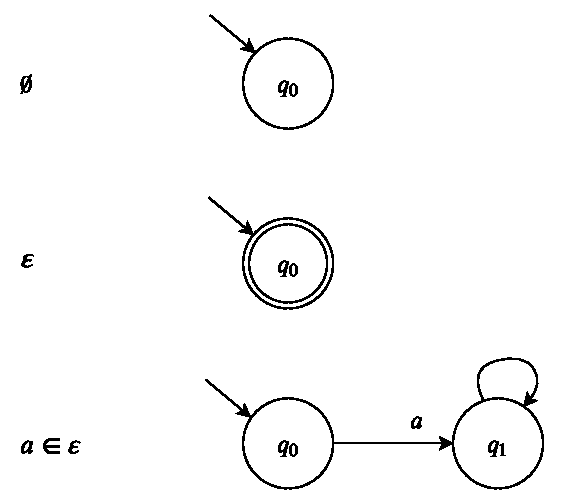
\includegraphics[scale=1]{16ottobre07.pdf}
\end{center}

Passo induttivo: Suppongo che $R$ e $S$ siano espressioni regolari -> $R$ e $S$ sono linguaggi.

\begin{center}
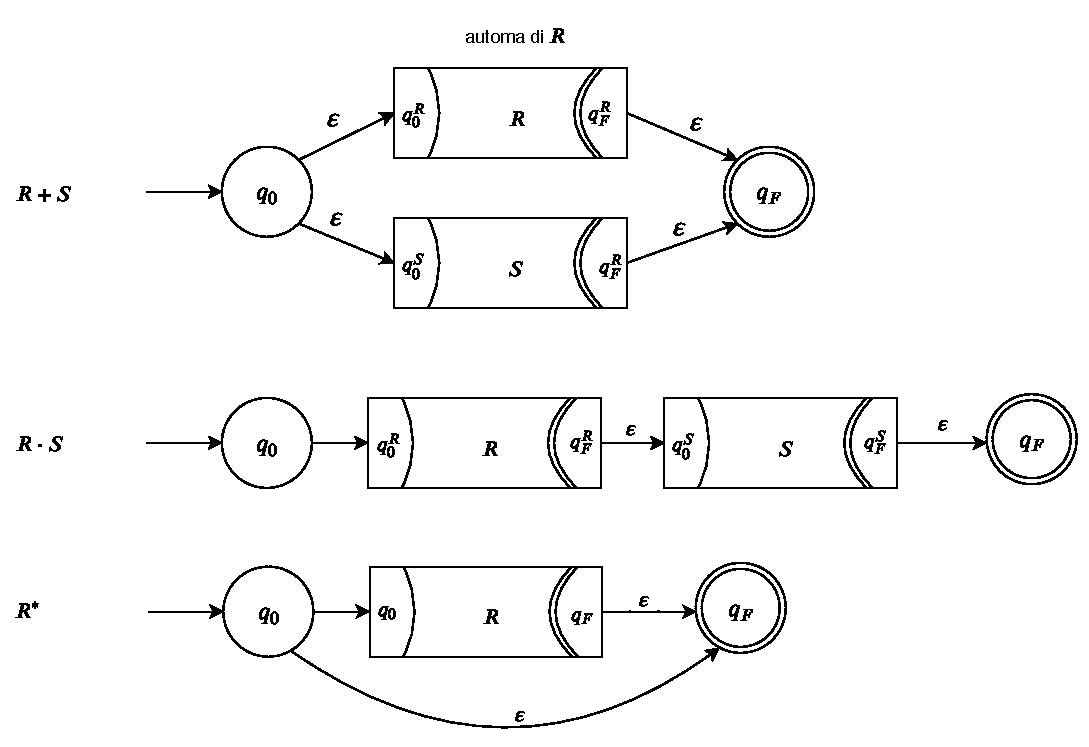
\includegraphics[scale=0.8]{16ottobre08.pdf}
\end{center}
\end{tcolorbox}

\noindent Per i linguaggi regolari valgono le seguenti proprietà:
\begin{itemize}
\item[-] $e_1 \cdot (e_2 + e_3)$ = $e_1e_2 + e_1e_3$. Lo stesso vale per $(e_1 \cdot e_2) \cdot e_3 $;
\item[-] $e_1 + (e_2 + e_3)$ = $(e_1 + e_2) + e_3$. Lo stesso vale per la moltiplicazione;
\item[-] $\emptyset^*$ = $\varepsilon$;
\item[-] $e^*+e$ = $e^*$;
\item[-] $(e^+)^*$ = $e^*$;
\item[-] $(e_1 + e_2)^*$ = $(e_1^*\cdot e_2^*)^*$;
\item[-] $e+\emptyset$ = $e$;
\item[-] $e \cdot \emptyset$ = $\emptyset \cdot e$ = $\emptyset$;
\end{itemize}


\end{document}